\chapter{DAH: Remote connection guide}
\label{sec:remote}

All of these techniques are tested as best we can, but rely on external software that may have its own problems.
If you have issues, please contact b.m.wynne@ed.ac.uk

\section{SSH connection to Raspberry Pi}

All Raspberry Pis in the DAH labs should be accessible via an SSH connection, assuming they are switched on.
To access one, first log into the Student Gateway machine:
\begin{verbatim}
  ssh -Y yourUUN@student.ph.ed.ac.uk
\end{verbatim}

Once you have logged into the Student Gateway (using your regular university username and password) you can now access the DAH labs.
\begin{verbatim}
  ssh -Y studentAA@dahpiBB
\end{verbatim}

For AA and BB you should substitute the student number you were given to login in the lab, and the number of the Pi that you were using.
Your login will work on any of the Pis, but please use the one you have been assigned unless it is not available.

Once you have access to the Pi, you should be able to retrieve or run any code that you have written.
If you are not familiar with the Linux command line, try using the ``nano'' editor to view or change files.

To download files from the Pi, it might be helpful to use FTP.
Log into the Student Gateway computer like before, but now connect to the Pi like this:
\begin{verbatim}
  sftp studentAA@dahpiBB
\end{verbatim}

You are now in a limited command-line environment that will respond to instructions like ``ls'' and ``cd'' to navigate the filesystem.
To download (for example) the file ``myTestFile.txt'' you would run the following command:
\begin{verbatim}
  get myTestFile.txt
\end{verbatim}

This file will now be available in your standard university account.
To close the connection to the Pi, or to the Student Gateway, simply type ``exit'' --- typing this while logged into the Pi will return you to the Student Gateway.


\section{Using a graphical interface remotely}

We do not support the option for you to run the full Pi desktop environment remotely.
However, you will be able to run programs with a GUI from the command line, and then see the GUI on your own machine.

If your own computer is running a Linux-based operating system then this will happen automatically, if you follow the instructions above.
You can test this by attempting to open a GUI-based program, such as ``geany'' the Python code editor.

If your computer is running Mac OS or Windows, you may need additional software, as described below.

\subsection{Windows}

(This information is based on \href{https://superuser.com/questions/119792/how-to-use-x11-forwarding-with-putty}{this webpage})

Viewing GUI programs from the Raspberry Pi in Windows will require you to have an SSH client that supports X-window forwarding, and an X-window server.
There are several options, but I strongly recommend using \href{https://www.putty.org/}{PuTTY} and \href{https://sourceforge.net/projects/vcxsrv/}{vcxsrv} as the client and server respectively.

Install both programs, and ensure that vcxsrv is running.
Now open PuTTY and configure it to allow X-window forwarding as shown:
\begin{center}
  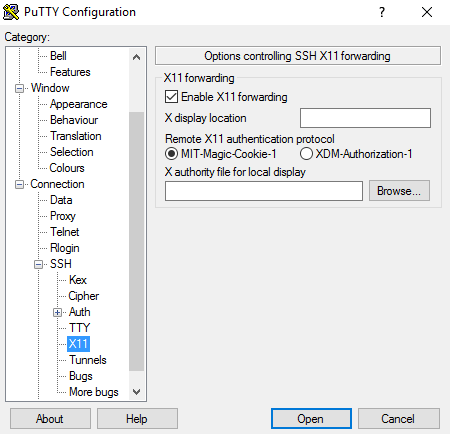
\includegraphics[width=14cm]{figs/PuttyXwin}
\end{center}

Use PuTTY to connect to the Student Gateway, and then follow the original instructions from that point.

\subsection{MacOS}

(This information is based on \href{https://www.youtube.com/watch?v=s6e3cqCISaE}{this video})

Viewing GUI programs from the Raspberry Pi in MacOS X will require you to install the \href{https://www.xquartz.org/}{XQuartz} application.
Once it is installed, start it running and open the Applications menu (you will not see anything other than the XQuartz menu bar at this point).
Select Terminal to create a new command line interface.
You can now follow the original instructions, connecting to the Student Gateway from within this terminal window.
